\documentclass[10pt]{beamer}

\mode<presentation>
{
  \usetheme[height=1.25cm]{Madrid}
  \setbeamertemplate{navigation symbols}{}
  \setbeamercolor{alerted text}{fg=illini}
}
\graphicspath{{./}{figs/}{/Users/hic/Dropbox/To-process/slides/pics/}{/Users/hic/Dropbox/To-process/slides/pics/feat-det/}{/Users/hic/Dropbox/To-process/slides/3630-08/}{/Users/hic/Dropbox/To-process/slides/8803-09/}{/Users/hic/Dropbox/To-process/slides/8803-12/}{/Users/hic/Dropbox/To-process/slides/8803-08/}}

\usebackgroundtemplate{
\includegraphics[width=\paperwidth,height=\paperheight]{uc-background}}

\usepackage[english]{babel}
\usepackage{epsfig,subfigure,bm}
\usepackage{multimedia}
\usepackage{psfrag}
\usepackage{animate}

% \usefonttheme{metropolis} % default family is serif
%%%%%% Begin of my macros and options

\setbeamertemplate{section in toc shaded}[default][55]
\setbeamertemplate{subsection in toc shaded}[default][55]
\setbeamercolor{block title}{fg=white,bg=illini}
\setbeamercolor{block body}{fg=black,bg=mygrey}

\setbeamercolor{emphprimary}{fg=CBlue}
\setbeamercolor{emphsecondary}{fg=illini}
\setbeamercolor{emphtertiary}{fg=mygreen}
\definecolor{darkForestGreen}{rgb}{.1,1,.1}
\definecolor{veryLightGray}{rgb}{.9,.9,.9}
\definecolor{greenApple}{rgb}{.3,.9,.3}

\setbeamercolor{title}{bg=CBlue}

\usepackage{amsmath,amssymb,amsxtra,amsthm}
\usepackage{algorithm,algorithmic}
\usepackage{natbib}
\usepackage{bibentry}
\usepackage{xspace}
\usepackage{changepage}

\definecolor{myblue}{rgb}{.2,.2,.7}
\definecolor{myred}{rgb}{.7,.2,.2}
\definecolor{mygreen}{rgb}{.2,.7,.2}
\definecolor{mygrey}{rgb}{0.9,0.9,0.9}
\definecolor{CBlue}{cmyk}{1,0.25,0,0}
\definecolor{illini}{rgb}{0.98,0.4,0.05}
\definecolor{black}{cmyk}{0,0,0,1}

\newcommand{\myemph}[1]{{\usebeamercolor[fg]{emphprimary}
    \textbf{#1}}}
\newcommand{\myemphalt}[1]{{\usebeamercolor[fg]{emphsecondary}
    \textbf{#1}}}


\title[Math for Robotics] % (optional, use only with long paper titles)
{CSE276C - Regression and Classification}

\author[H.~I. Christensen] % (optional, use only with lots of authors)
{Henrik I.~Christensen}
% - Give the names in the same order as the appear in the paper.  -
% Use the \inst{?} command only if the authors have different
% affiliation.

\AtBeginSection[]
{
   \begin{frame}
       \frametitle{Outline}
       \tableofcontents[currentsection]
   \end{frame}
}

\institute[UCSD] % (optional, but mostly needed)
{
  \begin{minipage}[c]{.2\textwidth}
    
\includegraphics[width=.65\linewidth]{ucsealnew}%
  \end{minipage}%
  \begin{minipage}[c]{.6\textwidth}
    \small
%%    \begin{center}
      Computer Science and Engineering\\
      University of California, San Diego\\
%%    \end{center}

  \end{minipage}
%%  \vspace*{1ex}
}
%% - Use the \inst command only if there are several affiliations.
%% - Keep it simple, no one is interested in your street address.

\bigskip

\date[Nov 2020]% (optional, should be abbreviation of conference name)
{\small%
  November 2020}

\begin{document}

\nobibliography{/Users/hic/Dropbox/bibliography/bib-file.bib}
\bibliographystyle{plain}

\begin{frame}[plain]
  \titlepage 
\end{frame}


\begin{frame}
  \frametitle{Introduction}
  \begin{itemize}
  \item Data science is a big part of robotics
  \item Many aspects of robotics rely on data analysis
    \begin{itemize}
    \item Recognition of objects
    \item Adpative Control
    \item Clean-up of sensor information
    \item ...
    \end{itemize}
  \end{itemize}
\end{frame}

\begin{frame}
  \frametitle{A general framework}
  \centerline{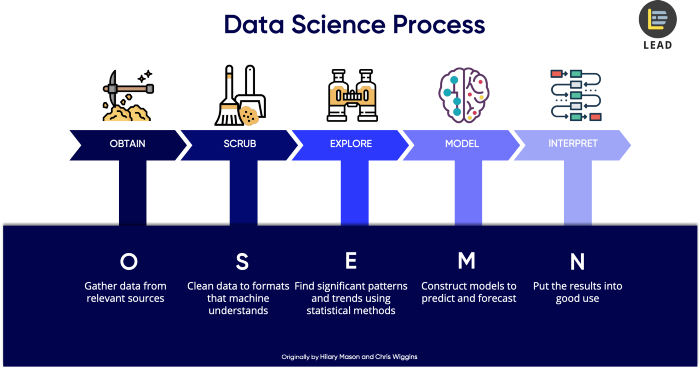
\includegraphics[width=12cm]{osemn}}
\end{frame}

\section{Introduction - Regression}
\begin{frame}
  \frametitle{Introduction}
  \begin{itemize}
  \item The objective of regression is to enable prediction of a value
    based on modeling over a dataset $X$.
  \item Consider a set of D observations over a space
  \item How can we generate estimates for the future?
    \begin{itemize}
    \item Battery time?
    \item Time to completion?
    \item Position of doors? 
    \end{itemize}
  \end{itemize}
\end{frame}

\begin{frame}
  \frametitle{Introduction (2)}
  \begin{itemize}
  \item Example
  \end{itemize}
  \begin{center}
    \includegraphics[height=5cm]{prml-Figure1-2}
    \[
    y(x,{\mathbf w}) = w_0 + w_1 x + w_2 x^2 + \ldots + w_m x^m =
                       \sum_{i=0}^m w_i x^i
    \]
  \end{center}
\end{frame}

\begin{frame}
  \frametitle{Introduction (3)}
  \begin{itemize}
  \item In general the functions could be beyond simple polynomials
  \item The ``components'' ($\phi_{i}(x)$) are termed {\em basis functions}, i.e. 
    \[
    y(x, {\mathbf w}) = \sum_{i=0}^m w_i \phi_i(x) = \vec{w}^T
    \vec{\phi(x)}
    \]
  \end{itemize}
\end{frame}

\section{Preliminaries}

\begin{frame}
  \frametitle{Loss Function}
  \begin{itemize}
  \item For optimization we need a penalty / loss function
    \[
    L(t, y(x))
    \]
  \item Expected loss is then
    \[
    E[L] = \int \int L(t,y(x)) p(x,t) dx dt
    \]
  \item For the squared loss function we have
    \[
    E[L] = \int \int \{ y(x) - t \}^2 p(x,t) dx dt
    \]
  \item Goal: choose y(x) to minimize expected loss (E[L])
  \end{itemize}
\end{frame}

\begin{frame}
  \frametitle{Loss Function}
  \begin{itemize}
  \item Derivation of the extrema
    \[ \frac{\delta E[L]}{\delta y(x)} = 2 \int \{ y(x) - t \} p(x,t) dt = 0
    \]
  \item Implies that
    \[
    y(x) = \frac{\int t p(x,t) dt}{p(x)} = \int t p(t|x) dt = E[t|x]
    \]
  \end{itemize}
\end{frame}

\begin{frame}
  \frametitle{Loss Function - Interpretation}
  \begin{center}
    \includegraphics[height=6cm]{prml-Figure1-28}
  \end{center}
\end{frame}

\begin{frame}
  \frametitle{Alternative}
  \begin{itemize}
  \item Consider a small rewrite
    \[
    \{y(x) - t\}^2 = \{ y(x) - E[t|x] + E[t|x] - t \}^2
    \]
  \item The expected loss is then
    \[
    E[L] = \int \{ y(x) - E[t|x]\}^2 p(x) dx +
           \int \{ E[t|x] - t\}^2 p(x) dx
    \]
  \end{itemize}
\end{frame}

\section[Linear Models]{Linear Basis Function Models}

\begin{frame}
  \frametitle{Polynomial Basis Functions}
  \begin{columns}
    \begin{column}{5cm}
      Basic Definition:
      \[
      \phi_i(x) = x^i
      \]
      Global functions\\
      Small change in x affects all of them
    \end{column}
    \begin{column}{5cm}
      \includegraphics[width=4.5cm]{prml-Figure3-1a}
    \end{column}
  \end{columns}
\end{frame}

\begin{frame}
  \frametitle{Gaussian Basis Functions}
  \begin{columns}
    \begin{column}{5cm}
      Basic Definition:
      \[
      \phi_i(x) = e^{- \frac{(x-\mu_i)^2}{2s^2}}
      \]
      A way to Gaussian mixtures, local impact\\
      Not required to have probabilistic interpretation.\\
      $\mu$ control position and $s$ control scale
    \end{column}
    \begin{column}{5cm}
      \includegraphics[width=4.5cm]{prml-Figure3-1b}
    \end{column}
  \end{columns}
\end{frame}

\begin{frame}
  \frametitle{Sigmoid Basis Functions}
  \begin{columns}
    \begin{column}{5cm}
      Basic Definition:
      \[
      \phi_i(x) = \sigma\left( \frac{x-\mu_i}{s} \right)
      \] where
      \[ \sigma(a) = \frac{1}{1+e^{-a}} \]
      \\
      $\mu$ controls location and $s$ controls slope
    \end{column}
    \begin{column}{5cm}
      \includegraphics[width=4.5cm]{prml-Figure3-1c}
    \end{column}
  \end{columns}
\end{frame}

\begin{frame}
  \frametitle{Maximum Likelihood \& Least Squares}
  \begin{itemize}
  \item Assume observation from a deterministic function contaminated
    by Gaussian Noise
    \[
    t = y(x,w) + \epsilon \quad p(\epsilon|\beta) =
    N(\epsilon|0,\beta^{-1})
    \]
    the problem at hand is then
    \[
    p(t|x,w,\beta) = N(t|y(x,w),\beta^{-1})
    \]
  \item From a series of observations we have the likelihood
    \[
    p({\mathbf t}| {\mathbf X}, w, \beta) = \prod_{i=1}^N N(t_i|w^T\phi(x_i),\beta^{-1})
    \]
  \end{itemize}
\end{frame}

\begin{frame}
  \frametitle{Maximum Likelihood \& Least Squares (2)}
  \begin{itemize}
  \item This results in 
    \[
    \ln p({\mathbf t}|{\mathbf w}, \beta ) = \frac{N}{2} \ln \beta -
    \frac{N}{2} \ln (2\pi) - \beta E_D({\mathbf w})
    \]
  \item where
    \[
    E_D({\mathbf w}) = \frac{1}{2} \sum_{i=1}^{N} \{ t_i - {\mathbf
      w}^T{\mathbf \phi}(x_i)\}^2
    \]
    is the sum of squared errors
  \end{itemize}
\end{frame}

\begin{frame}
  \frametitle{Maximum Likelihood \& Least Squares (3)}
  \begin{itemize}
  \item Computing the extrema yields:
    \[
    {\mathbf w}_{ML} = \left( \Phi^T \Phi \right)^{-1} \Phi^T
    {\mathbf t}
    \]
  \item where
    \[
    \Phi = \left(
      \begin{array}{cccc}
        \phi_0(x_1) & \phi_1(x_1) & \cdots & \phi_{M-1}(x_1) \\
        \phi_0(x_1) & \phi_1(x_2) & \cdots & \phi_{M-1}(x_2) \\
        \vdots      & \vdots      & \ddots & \vdots         \\
        \phi_0(x_N) & \phi_1(x_N) & \cdots & \phi_{M-1}(x_N) \\
      \end{array}
    \right)
    \]
  \end{itemize}
\end{frame}

\begin{frame}
  \frametitle{Line Estimation}
  \begin{itemize}
  \item Least square minimization:
    \begin{itemize}\setlength{\itemsep}{0pt}
    \item Line equation: $y=a x + b$
    \item Error in fit: $\sum_i (y_i - a x_i - b)^2$
    \item Solution: \[
      \left( \begin{array}{c} \bar{y^2}\\ \bar{y} \end{array}
      \right) = \left( \begin{array}{cc}
          \bar{x^2} & \bar{x} \\
          \bar{x}   & 1\\ \end{array} \right) \left(
        \begin{array}{c} a \\ b \end{array} \right)
      \]
    \item So what is the problem? \pause
    \item Minimizes vertical errors. Non-robust!
    \end{itemize}
  \end{itemize}
\end{frame}

\begin{frame}
  \frametitle{LSQ on Lasers}
  \begin{itemize}
  \item Line model: $r_i \cos(\phi_i - \theta) = \rho$
  \item Error model: $d_i = r_i \cos(\phi_i - \theta) - \rho$
  \item Optimize: $ \textrm{argmin}_{(\rho,\theta)} \sum_i (r_i
    \cos(\phi_i - \theta) - \rho)^2 $
  \item Error model derived in \citet{Deriche92a}
  \item Well suited for ``clean-up'' of Hough lines
  \end{itemize}
\end{frame}

\begin{frame}
  \frametitle{Total Least Squares}
  \begin{itemize}
  \item Line equation: $ a x + b y + c = 0 $
  \item Error in fit: $ \sum_i (a x_i + b y_i + c)^2 $ where $a^2
    + b^2 = 1$. 
  \item Solution: \[
    \left( \begin{array}{cc}
        \bar{x^2} - \bar{x}\bar{x} & \bar{xy} - \bar{x}\bar{y} \\
        \bar{xy} - \bar{x}\bar{y}  & \bar{y^2} - \bar{y}\bar{y}\\
      \end{array} \right) 
    \left( \begin{array}{c}
        a \\ b \end{array} \right) = \mu 
    \left( \begin{array}{c}
        a \\ b \end{array} \right) \] where $\mu$ is a scale
    factor.
  \item $c = -a \bar{x} - b \bar{y}$
  \end{itemize}
\end{frame}

\begin{frame}
  \frametitle{Line Representations}
  \begin{columns}
    \begin{column}{5.5cm}
      \includegraphics[width=5.5cm]{line-rep}
    \end{column}
    \begin{column}{6cm}
      \begin{itemize}\setlength{\itemsep}{0pt}
      \item The line representation is crucial
      \item Often a redundant model is adopted
      \item Line parameters vs end-points
      \item Important for fusion of segments.
      \item End-points are less stable 
      \end{itemize}
    \end{column}
  \end{columns}
\end{frame}


\begin{frame}
  \frametitle{Sequential Adaptation}
  \begin{itemize}
  \item In some cases one at a time estimation is more suitable
  \item Also known as gradient descent
    \begin{eqnarray*}
      {\mathbf w}^{(\tau+1)} &=& {\mathbf w}^{(\tau)} - \eta \nabla E_n\\
                             &=& {\mathbf w}^{(\tau)} - \eta (t_n -
                             {\mathbf w}^{(\tau)T} \phi(x_n))
                             \phi(x_n)
    \end{eqnarray*}
  \item Knows as least-mean square (LMS). An issue is how to choose
    $\eta$?
  \end{itemize}
\end{frame}

\begin{frame}
  \frametitle{Regularized Least Squares}
  \begin{itemize}
  \item As seen in previous lecture sometime control of parameters might be
    useful.
  \item Consider the error function:
    \[
    E_D({\mathbf w}) + \lambda E_W({\mathbf w})
    \]
  \item which generates
    \[
    \frac{1}{2}\sum_{i=1}^N \{ t_i - w^t\phi(x_i)\}^2 +
    \frac{\lambda}{2} {\mathbf w}^T{\mathbf w}
    \]
  \item which is minimized by 
    \[
    w = \left( \lambda I + \Phi^T \Phi \right)^{-1} \Phi^T {\mathbf t}
    \]
  \end{itemize}
\end{frame}


\section[Bayes Regress]{Bayesian Linear Regression}

\begin{frame}
  \frametitle{Bayesian Linear Regression}
  \begin{itemize}
  \item Define a conjugate prior over $w$
    \[
    p(w) = N(w|m_0,S_0)
    \]
  \item given the likelihood function and regular from Bayesian
    analysis we can derive
    \[
    p(w|t) = N(w|m_N, S_N)
    \]
  \item where
    \begin{eqnarray*}
      m_N & = & S_N\left(S_0^{-1}m_0+ \beta \Phi^T t\right) \\
      S_N^{-1} & = & S_0^{-1} + \beta \Phi^T \Phi
    \end{eqnarray*}
  \end{itemize}
\end{frame}

\begin{frame}
  \frametitle{Bayesian Linear Regression (2)}
  \begin{itemize}
  \item A common choice is
    \[
    p(w) = N(w|0, \alpha^{-1} I)
    \]
  \item So that
    \begin{eqnarray*}
      m_N & =& \beta S_N \Phi^T t\\
      S_N^{-1} &=& \alpha I + \beta \Phi^T \Phi
    \end{eqnarray*}
  \end{itemize}
\end{frame}

\begin{frame}
  \frametitle{Example - No Data}
  \begin{center}
    \includegraphics[width=10cm]{prml-Figure3-7a}
  \end{center}
\end{frame}

\begin{frame}
  \frametitle{Example - 1 Data Point}
  \begin{center}
    \includegraphics[width=10cm]{prml-Figure3-7b}
  \end{center}
\end{frame}

\begin{frame}
  \frametitle{Example - 2 Data Points}
  \begin{center}
    \includegraphics[width=10cm]{prml-Figure3-7c}
  \end{center}
\end{frame}

\begin{frame}
  \frametitle{Example - 20 Data Points}
  \begin{center}
    \includegraphics[width=10cm]{prml-Figure3-7d}
  \end{center}
\end{frame}

\section[Model Comparison]{Bayesian Model Comparison}


\begin{frame}
  \frametitle{Bayesian Model Comparison}
  \begin{itemize}
  \item How does one select an appropriate model?
  \item Assume for a minute we want to compare a set of models $M_i$,
    $i \in 1, ... L$ for a dataset D
  \item We could compute
    \[
    p(M_i | D) \propto p(D | M_i) p(M_i)
    \]
  \item Bayes Factor: Ratio of evidence for two models
    \[
    \frac{p(D | M_i )}{p(D | M_j)}
    \]
  \end{itemize}
\end{frame}

\begin{frame}
  \frametitle{The mixture distribution approach}
  \begin{itemize}
  \item We could use all the models:
    \[
    p(t|x,D) = \sum_{i=1}^L p(t|x,M_i,D) p(M_i|D)
    \]
  \item Or simply go with the most probably/best model. 
  \end{itemize}
\end{frame}

\begin{frame}
  \frametitle{Model Evidence}
  \begin{itemize}
  \item We can compute model evidence
    \[
    p(D|M_i) = \int p(D|w, M_i) p(w|M_i) dw
    \]
  \item Allow computation of model fit based on parameter range 
  \end{itemize}
\end{frame}

\begin{frame}
  \frametitle{Evaluation of Parameters}
  \begin{itemize}
  \item Evaluation of posterior over parameters
    \[ p(w | D, M_i) = \frac{ P(D | w, M_i) p(w | M_i)}{P(D|M_i)} \]
  \item There is a need to understand how good is a model?
  \end{itemize}
\end{frame}

\begin{frame}
  \frametitle{Model Comparison}
  \begin{itemize}
  \item Consider evaluation of a model w. parameters w
    \[ 
    p(D) = \int p(D|w) p(w) dw \approx p(D|w_{map})
    \frac{\sigma_{posterior}}{\sigma_{prior}}
    \]
  \item Then
    \[
    \ln p(D) \approx \ln p(D|w_{map}) + \ln
    \left( \frac{\sigma_{posterior}}{\sigma_{prior}} \right)
    \]
  \end{itemize}
\end{frame}

\begin{frame}
  \frametitle{Model Comparison as Kullback-Leibler}
  \begin{itemize}
  \item From earlier we have comparison of distributions
    \[
    KL = \int p(D|M_1) \ln \frac{p(D|M_1)}{p(D|M_2)} d D
    \]
  \item Enables comparison of two different models
  \end{itemize}
\end{frame}


\section{Regression Summary}

\begin{frame}
  \frametitle{Regression Summary}
  \begin{itemize}
  \item Brief intro to linear methods for estimation of models
  \item Prediction of values and models
    \begin{itemize}
    \item Needed for adaptive selection of models (black-box/grey-box)
    \item Evaluation of sensor models, \ldots
    \end{itemize}
  \item Consideration of batch and recursive estimation methods
  \item Significant discussion of methods for evaluation of models and
    parameters.
  \item This far purely a discussion of linear models
  \end{itemize}
\end{frame}


\section{Classification}

\begin{frame}
  \frametitle{Classification Introduction}
  \begin{itemize}
  % \item Last time: prediction of new functional values
  \item Linear classification of data
    \begin{itemize}
    \item Basic pattern recognition
    \item Separation of data: buy/sell
    \item Segmentation of line data, \ldots
    \end{itemize}
  \end{itemize}
\end{frame}

\begin{frame}
  \frametitle{Simple Example - Bolts or Needles}
  \begin{center}
    \includegraphics[height=7cm]{class1}
  \end{center}
\end{frame}

\begin{frame}
  \frametitle{Classification}
  \begin{itemize}
  \item Given 
    \begin{itemize}
    \item An input vector: $X$
    \item A set of classes: $c_i \in {\cal C}, \quad i=1, \ldots, k$
    \end{itemize}
  \item Mapping $m: X \rightarrow {\cal C}$
  \item Separation of space into decision regions
  \item Boundaries termed decision boundaries/surfaces
  \end{itemize}
\end{frame}

\begin{frame}
  \frametitle{Basis Formulation}
  \begin{itemize}
  \item It is a 1-of-K coding problem
  \item Target vector: ${\mathbf t} =\left( 0, \ldots, 1, \ldots, 0
    \right)$
  \item Consideration of 3 different approaches
    \begin{enumerate}
    \item Optimization of discriminant function
    \item Bayesian Formulation: $p(c_i | x)$
    \item Learning \& Decision fusion
    \end{enumerate}
  \end{itemize}
\end{frame}

\begin{frame}
  \frametitle{Code for experimentation}
  \begin{itemize}
  \item There are data sets and sample code available
    \begin{itemize}
    \item NETLAB: \url{http://www.ncrg.aston.ac.uk/netlab/index.php}
    \item Kaggle: \url{https://www.kaggle.com}
    \item Lots of good robotics datasets too
    \end{itemize}
  \end{itemize}
\end{frame}


\section[Disc. Func.]{Linear Discriminant Functions}


\begin{frame}
  \frametitle{Discriminant Functions}
  \begin{itemize}
  \item Objective: input vector $x$ assigned to a class $c_i$
  \item Simple formulation:
    \[ y({\mathbf x}) = {\mathbf w}^T {\mathbf x} + w_0 \]
  \item $\mathbf w$ is termed a weight vector
  \item $w_0$ is termed a bias
  \item Two class example: $c_1$ if $y({\mathbf x}) \geq 0$ otherwise $c_2$
  \end{itemize}
\end{frame}

\begin{frame}
  \frametitle{Basic Design}
  \begin{itemize}
  \item Two points on decision surface ${\mathbf x}_a$ and ${\mathbf x}_b$
  \item $y({\mathbf x}_a) = y({\mathbf x}_b) = 0 \Rightarrow {\mathbf w}^T
    ({\mathbf x}_a - {\mathbf x}_b) = 0$
  \item ${\mathbf w}$ perpendicular to decision surface
    \[
    \frac{ {\mathbf w}^T {\mathbf x}}{|| {\mathbf w} ||} = -
    \frac{w_0}{|| {\mathbf w} ||} 
    \]
  \item Define: $\tilde{w} = (w_0, {\mathbf w})$ and $\tilde{x} =
    (1, {\mathbf x})$ so that:
    \[ y( {\mathbf x} ) = \tilde{w}^T \tilde{x} \]
  \end{itemize}
\end{frame}

\begin{frame}
  \frametitle{Linear discriminant function}
  \begin{center}
    \includegraphics[height=6cm]{prml-Figure4-1}
  \end{center}
\end{frame}

\begin{frame}
  \frametitle{Multi Class Discrimination}
  \begin{itemize}
  \item Generation of multiple decision functions
    \[
    y_k({\mathbf x}) = {\mathbf w}_k^T {\mathbf x} + w_{k0}
    \]
  \item Decision strategy
    \[
    j = \arg \max_{i\in 1..k} y_i({\mathbf x})
    \]
  \end{itemize}
\end{frame}

\begin{frame}
  \frametitle{Multi-Class Decision Regions}
  \begin{center}
    \includegraphics[height=6cm]{prml-Figure4-3}
  \end{center}
\end{frame}


\begin{frame}
  \frametitle{Example - Bolts or Needles}
  \begin{center}
    \includegraphics[height=7cm]{class1}
  \end{center}
\end{frame}

\begin{frame}
  \frametitle{Minimum distance classification}
  \begin{itemize}
  \item Suppose we have computed the mean value for each of the classes
  \item $m_{needle} = [0.86, 2.34]^T$ and $m_{bolt} = [5.74, 5,85]^T$
  \item We can then compute the minimum distance
    \[ d_j(x) = || x - m_j || \]
  \item ${\mathrm argmin}_i d_i(x)$ is the best fit
  \item Decision functions can be derived
  \end{itemize}
\end{frame}

\begin{frame}
  \frametitle{Bolts / Needle Decision Functions}
  \begin{description}
  \item[Needle] $d_{needle}(x) = 0.86 x_1 + 2.34 x_2 - 3.10 $
  \item[Bolt]   $d_{bolt}(x) = 5.74 x_1 + 5.85 x_2 - 33.59$
  \item Decision boundary
    \[ d_i(x) - d_j(x) = 0 \]
  \item $d_{needle/bolt}(x) = -4.88 x_1 - 3.51 x_2 + 30.49$
  \end{description}
\end{frame}

\begin{frame}
  \frametitle{Example decision surface}
  \begin{center}
    \includegraphics[height=7cm]{class3}
  \end{center}
\end{frame}



\section{LSQ for Classification}

\begin{frame}
  \frametitle{Least Squares for Classification}
  \begin{itemize}
  \item Just like we could do LSQ for regression we can perform an
    approximation to the classification vector ${\cal C}$
  \item Consider again
    \[
    y_k({\mathbf x}) = {\mathbf w}_k^T {\mathbf x} + w_{k0}
    \]
  \item Rewrite to 
    \[
    {\mathbf y}({\mathbf x}) = \tilde{{\mathbf W}}^T \tilde{{\mathbf x}}
    \]
  \item Assuming we have a target vector ${\mathbf T}$
  \end{itemize}
\end{frame}

\begin{frame}
  \frametitle{Least Squares for Classification}
  \begin{itemize}
  \item The error is then:
    \[
    E_D(\tilde{\mathbf W}) = \frac{1}{2} Tr\left\{ (\tilde{\mathbf
        X}\tilde{\mathbf W} - {\mathbf T})^T(\tilde{\mathbf
        X}\tilde{\mathbf W} - {\mathbf T})\right\}
    \]
  \item The solution is then
    \[
    \tilde{\mathbf W} = \left( \tilde{\mathbf X}^T \tilde{\mathbf X}
    \right)^{-1} \tilde{\mathbf X}^T {\mathbf T}
    \]
  \end{itemize}
\end{frame}

\begin{frame}
  \frametitle{LSQ and Outliers}
  \begin{center}
    \begin{tabular}[c]{cc}
      \includegraphics[width=5.5cm]{prml-Figure4-4a} &
      \includegraphics[width=5.5cm]{prml-Figure4-4b}
    \end{tabular}
  \end{center}
\end{frame}

\section[Fisher's Method]{Fisher's Discriminant Method}


\begin{frame}
  \frametitle{Fisher's linear discriminant}
  \begin{itemize}
  \item Selection of a decision function that maximizes distance
    between classes
  \item Assume for a start
    \[
    y = {\mathbf W}^T {\mathbf x}
    \]
  \item Compute $m_1$ and $m_2$
    \[
    \begin{array}[c]{cc}
      {\mathbf m}_1 = \frac{1}{N_1}\sum_{i\in C_1} {\mathbf x}_i &
      {\mathbf m}_2 = \frac{1}{N_2}\sum_{j\in C_2} {\mathbf x}_j
    \end{array}
    \]
  \item Distance:
    \[
    m_2 - m_1 = {\mathbf w}^T \left( {\mathbf m}_2 - {\mathbf m}_1
    \right)
    \]
  \item where $m_i = {\mathbf w} {\mathbf m}_i$
  \end{itemize}
\end{frame}

\begin{frame}
  \frametitle{The suboptimal solution}
  \begin{center}
    \includegraphics[height=6cm]{prml-Figure4-6a}
  \end{center}
\end{frame}

\begin{frame}
  \frametitle{The Fisher criterion}
  \begin{itemize}
  \item Consider the expression
    \[
    J(w) = \frac{{\mathbf w}^T {\mathbf S}_B {\mathbf w}}{{\mathbf
        w}^T {\mathbf S}_W {\mathbf w}}
    \]
  \item where ${\mathbf S}_B$ is the between class covariance and
    ${\mathbf S}_W$ is the within class covariance, i.e.
    \[ 
    {\mathbf S}_B = ( {\mathbf m}_1 - {\mathbf m}_2 )( {\mathbf m}_1 -
    {\mathbf m}_2 )^T
    \]
    and
    \[
    {\mathbf S}_W = \sum_{i={\cal C}_1}
    ({\mathbf x}_i - {\mathbf m}_1)({\mathbf x}_i - {\mathbf m}_1)^T
    + \sum_{i={\cal C}_2}
    ({\mathbf x}_i - {\mathbf m}_2)({\mathbf x}_i - {\mathbf m}_2)^T
    \]
  \item Optimized when
    \[
    ({\mathbf w}^T {\mathbf S}_B {\mathbf w}) {\mathbf S}_w {\mathbf
      w} = ({\mathbf w}^T {\mathbf S}_W {\mathbf w}) {\mathbf S}_B
    {\mathbf w}
    \] 
    or
    \[
    {\mathbf w} \propto {\mathbf S}_w^{-1} ({\mathbf m}_2 - {\mathbf
      m}_1)
    \]
  \end{itemize}
\end{frame}

\begin{frame}
  \frametitle{The Fisher result}
  \begin{center}
    \includegraphics[height=6cm]{prml-Figure4-6b}
  \end{center}
\end{frame}

\begin{frame}
  \frametitle{Generalization to $N > 2$}
  \begin{itemize}
  \item Define a stacked weight factor
    \[
    {\mathbf y} = {\mathbf W}^T {\mathbf x}
    \]
  \item The within class covariance generalizes to
    \[
    {\mathbf S}_w = \sum_{k=1}^K {\mathbf S}_k
    \]
  \item The between class covariance is
    \[
    {\mathbf S}_B = \sum_{k=1}^K N_k ({\mathbf m_k} - {\mathbf
      m})({\mathbf m_k} - {\mathbf m})^T
    \]
  \item It can be shown that $J({\mathbf w})$ is optimized by the
    eigenvectors to the equation
    \[
    S = {\mathbf S}_W^{-1} {\mathbf S}_B
    \]
  \end{itemize}
\end{frame}


\section{Perceptrons}

\begin{frame}
  \frametitle{Perceptron Algorithm}
  \begin{itemize}
  \item Developed by Rosenblatt (1962)
  \item Formed an important basis for neural networks
  \item Use a non-linear transformation $\phi(x)$
  \item Construct a decision function
    \[
    y({\mathbf x}) = f\left( {\mathbf w}^T \phi({\mathbf x}) \right)
    \]
  \item where\@
    \[
    f(a) = \left\{
      \begin{array}[c]{cc}
        +1, & a\geq 0 \\
        -1, & a < 0
      \end{array} \right.
    \]
  \end{itemize}
\end{frame}

\begin{frame}
  \frametitle{The perceptron criterion}
  \begin{itemize}
  \item Normally we want\@
    \[
    w^t \phi(x_n) > 0
    \]
  \item Given the target vector definition
    \[
    E_p({\mathbf w}) = - \sum_{n \ in {\cal M}} {\mathbf w}^T \phi_n t_n
    \]
  \item Where ${\cal M}$ represents all the mis-classified samples
  \item We can make this a gradient descent as seen in last lecture
    \[
    {\mathbf w}^{(\tau+1)} = {\mathbf w}^{(\tau)} - \eta \nabla E_P({\mathbf w})
                         = {\mathbf w}^{(\tau)} + \eta \phi_n t_n
    \]
  \end{itemize}
\end{frame}

\begin{frame}
  \frametitle{Perceptron learning example}
  \begin{center}
    \begin{tabular}[c]{cc}
      \includegraphics[height=3cm]{prml-Figure4-7a} &
      \includegraphics[height=3cm]{prml-Figure4-7b} \\
      \includegraphics[height=3cm]{prml-Figure4-7c} & 
      \includegraphics[height=3cm]{prml-Figure4-7d} \\
    \end{tabular}
  \end{center}
\end{frame}

\section{Summary}

\begin{frame}
  \frametitle{Classification Summary}
  \begin{itemize}
  \item Basics for discrimination / classification
  \item Obviously not all problems are linear
  \item Optimization of the distance/overlap between classes
    \begin{itemize}
    \item Minimizing the probability of error classification 
    \end{itemize}
  \item Basic formulation as an optimization problem
  \item How to optimize between cluster distance? Covariance Weighted
  \item Basic recursive formulation
  \item Could we make it more robust? 
  \end{itemize}
\end{frame}

\begin{frame}
  \frametitle{Summary}
  \begin{itemize}
  \item Data models are anchored in pure data driven or model based evaluation
  \item How can we use models to interpret data and extrapolate beyond the basic data?
  \item Covered basic models for regression and classification. 
  \end{itemize}
\end{frame}

% \bibliographystyle{acm}

\end{document}

%%% Local Variables:
%%% mode: latex
%%% TeX-master: t
%%% End:
